\section{The \texorpdfstring{$\nim{2}$}{*2} Question}\label{sec:star2}

\subsection{The Textbook Candidate}

\begin{figure}[!t]
\centering
\begin{subfigure}{0.32\columnwidth}\centering
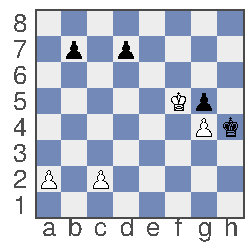
\includegraphics[width=\linewidth]{figures/star2_textbook.pdf}
\caption{Candidate}\label{fig:star2_textbook}
\end{subfigure}\hfill
\begin{subfigure}{0.32\columnwidth}\centering
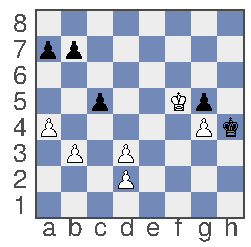
\includegraphics[width=\linewidth]{figures/star2_seven_a.pdf}
\caption{Position A}\label{fig:star2_seven_a}
\end{subfigure}\hfill
\begin{subfigure}{0.32\columnwidth}\centering
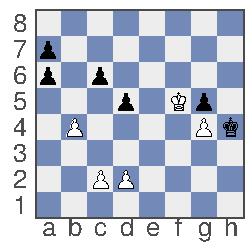
\includegraphics[width=\linewidth]{figures/star2_seven_b.pdf}
\caption{Position B}\label{fig:star2_seven_b}
\end{subfigure}
\caption{Positions of the $\nim{2}$ question beside T (Fig.~\ref{fig:trebuchet}; ordinary board). (a)~Candidate:
$\nim{2}$ under the textbook test, $\game{2\pm1}{-2\pm1}$ under the e.p.-aware test. (b)~Position A and
(c)~position B: $\nim{2}$ in the default setting.}
\label{fig:star2}
\end{figure}

The candidate \pos{W a2 c2 / B b7 d7} (Fig.~\ref{fig:star2_textbook}) is, under the count rule with the
textbook test, the only $\nim{k}$ with $k\ge2$ in the census: a2--a4 and c2--c4 leave $\star$ and $0$, and by
symmetry black's d7--d5 and b7--b5 do the same, so $G=\game{0,\star}{0,\star}=\nim{2}$. Its weak point is
black's b7--b5 and b5--b4: the textbook test then scores a2--a4 as $+\BIG$, but black takes b4$\times$a3 en
passant (Fig.~\ref{fig:basic}(a)). Under the e.p.-aware test \pos{W a2 c2 / B b4 d7} is worth $-3$, b7--b5 is
worth $-2\pm1$ and, by symmetry, c2--c4 is worth $2\pm1$; the other moves are dominated or reversible, so
$G=\game{2\pm1}{-2\pm1}$, a hot game with mean $0$ and temperature $2$ \lab{C2} (Section~S6 gives the details).

\subsection{No \texorpdfstring{$\nim{2}$}{*2} With Six Pawns or Fewer}

\begin{theorem}[Census; \lab{C2}]\label{thm:census}
In the census of Section~\ref{sec:atlas}, in the default setting, no position has value $\nim{k}$ with
$k\ge2$; the census has $6{,}724$ zeros and $4{,}042$ stars.
\end{theorem}

Our CGT engine and an independent C solver agree on every record, and the independent whole-board solver
finds no $\nim{k}$ with $2\le k\le 292$ among $793{,}299$ labeled placements on widths 1--4; every position in
scope has birthday at most $292$. Under the textbook test the census has $6{,}470$ zeros, $3{,}891$ stars and the candidate.

\subsection{\texorpdfstring{$\nim{2}$}{*2} With Seven Pawns}

\begin{theorem}[$\nim{2}$ with seven pawns; \lab{C2}]\label{thm:star2seven}
In the default setting, position~A, \pos{W a4 b3 d2 d3 / B a7 b7 c5}, and position~B,
\pos{W b4 c2 d2 / B a6 a7 c6 d5}, on files a--d of the ordinary board, have value $\nim{2}$. Neither is $\nim{2}$
with e.p.\ off or under the opponent rule.
\end{theorem}

Both fit beside T, and their pawns can arise in a game (Section~S6). In position A (Fig.~\ref{fig:star2_seven_a}), if white moves first, a4--a5 leaves $0$. The move d3--d4 attacks
c5; every black reply except c5$\times$d4 loses at once, and after c5$\times$d4 white continues b3--b4 to
$\star$, so the reversible move d3--d4 counts as a move to $\star$. White's third move, b3--b4, loses to
c5$\times$b4. If black moves first, a7--a5 leaves $0$ and b7--b6 leaves $\star$. Black's other moves are
reversible: after a7--a6 and b7--b5 white has replies worth $2$ and $3$, both at least $G$; and c5--c4
lets d3$\times$c4 free white's d2 pawn for $+\BIG$. Thus $G=\game{0,\star}{0,\star}=\nim{2}$. Position B is A
with the colors reversed and the files mirrored, and its analysis matches move for move (Section~S6).

\begin{table}[!t]
\centering
\caption{Values of the Candidate and of Positions A and B in the Model Settings}
\label{tab:star2_settings}
\footnotesize
\setlength{\tabcolsep}{4pt}
\begin{tabular}{@{}lccc@{}}
\toprule
Race rule, passed-pawn test & Candidate & A & B\\
\midrule
count, e.p.-aware & $\game{2\pm1}{-2\pm1}$ & $\nim{2}$ & $\nim{2}$\\
mover, e.p.-aware & $\game{2\pm1}{-2\pm1}$ & $\nim{2}$ & $\nim{2}$\\
count or mover, textbook & $\nim{2}$ & $\nim{2}$ & $\nim{2}$\\
count or mover, e.p.\ off & $\nim{2}$ & not $\nim{2}$ & not $\nim{2}$\\
opponent, any e.p.\ option & $0$ & not $\nim{2}$ & not $\nim{2}$\\
\bottomrule
\end{tabular}
\end{table}

In Table~\ref{tab:star2_settings} (e.p.\ on unless stated) every entry is \lab{C2}; for A and B, three
programs agree on each. The candidate needs the textbook test but survives e.p.\ off; A and B need en passant
but not the textbook test.

\subsection{Counts}\label{sec:star2-five}

On ordinary boards of width at most four, in the default setting, two $\nim{2}$ positions, A and B, have seven
pawns and four have eight; one exhaustive scan of $5{,}503{,}282$ root positions gives these counts \lab{C1},
and our engine re-checked every one \lab{C2}. With Theorem~\ref{thm:census}, seven is the least number of pawns
in a $\nim{2}$ on these boards \lab{C2}. A whole-board scan of every position with at most seven
pawns on up to nine files extends this to ordinary boards of any width (Section~S6): it finds no $\nim{k}$ with $k\ge2$ with six pawns or
fewer, and the only seven-pawn $\nim{2}$ are A and B \lab{C2}; Section~S6 gives the counts on five files.

\subsection{Rings and Higher Nimbers}\label{sec:star2-rings}

\begin{figure}[!t]
\centering
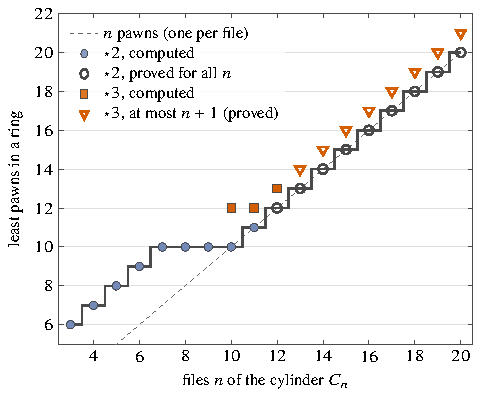
\includegraphics{figures/f2_least_pawns.pdf}
\caption{Least number of pawns in a ring of value $\nim{2}$ (steps) and $\nim{3}$ on $\cyl{n}$, in the default
setting. Filled markers are computed minima (\lab{C2} for $\nim{2}$, \lab{C1} for $\nim{3}$), open ones proved for all
$n$ as whole-board games \lab{S}; open triangles are upper bounds. The dashed line is one pawn per file. $\nim{3}$ is plotted from $n=10$;
ten-pawn $\nim{3}$ rings also exist on $\cyl{7}$ and $\cyl{8}$.}
\label{fig:least}
\end{figure}

Fig.~\ref{fig:least} gives the least ring $\nim{2}$ and $\nim{3}$ on each cylinder; Section~S6 lists example rings, counts and checks for every $n$. The first ring $\nim{2}$ on
$\cyl{n}$ has $n+3$ pawns for $n=3,\dots,7$ \lab{C2}, among them the six-pawn \pos{W a2 a3 b2 / B b7 c6 c7} on
$\cyl{3}$, one pawn fewer than any ordinary board of width at most four allows; it needs two en passant
captures, and with e.p.\ off it is $0$ \lab{C2}. On $\cyl{8}$ and $\cyl{9}$ ten is again the least \lab{C2}.
From $\cyl{10}$ on, one pawn per file, the least a ring can have, suffices: \pos{W b2 d2 e3 h3 j5 / B a4 c6 f6
g7 i7} on $\cyl{10}$ (the ring $M_{10}$ of Fig.~\ref{fig:ring}) and \pos{W c5 e3 h3 i2 k2 / B a4 b7 d7 f7 g6 j6}
on $\cyl{11}$ are $\nim{2}$ \lab{C2}.

For proofs we use \emph{walls}: runs of files with one pawn each, alternating in color, the black pawn two
ranks above the white (B4, W2: a black pawn on rank 4, a white one on rank 2). If a wall pawn moves, its neighbor
captures it and gets a passed pawn, so wall moves lose; with them deleted, inserting a pair of wall files leaves
the \emph{reduced game}, played in a window of five or six files, unchanged. As a whole-board game this gives a
ring $\nim{2}$ with $n+3$ pawns on every $\cyl{n}$ with $n\ge5$ \lab{S}, checked by two programs for $n<17$
\lab{C2}, and as sums of components our engine confirms it only to $n=12$ \lab{C1}. The same argument proves the
two $n$-pawn families above $\nim{2}$ as whole-board games for every $n\ge10$ \lab{S}; as sums of
components they are $\nim{2}$ on $\cyl{10}$ and $\cyl{11}$ \lab{C1}.

A $\nim{3}$ lies just beyond these scans, as a single component with nine pawns: B with a white a2 and a black a4
added, \pos{W a2 b4 c2 d2 / B a4 a6 a7 c6 d5}, is $\nim{3}$ on four files \lab{C2}. In the whole-board game no
position with eight pawns or fewer on up to eight files, ordinary or cylinder, is $\nim{3}$ \lab{C1}. On
$\cyl{7}$ eight ten-pawn rings are $\nim{3}$ \lab{C2}. Wall insertion gives a whole-board $\nim{3}$ with $n+2$
pawns on every $\cyl{n}$ with even $n\ge8$ and odd $n\ge11$, and with $n+1$ pawns on every $\cyl{n}$ with
$n\ge12$ \lab{S}. Height matters: on boards of three to five files, seven ranks give a $\nim{2}$ with four
pawns, \pos{W a2 c2 / B c3 b6}, and a $\nim{3}$ with six; six ranks give a $\nim{2}$ and five give none
\lab{C2}. But no $\nim{4}$ has turned up:
none of the $134{,}920{,}191$ one-component ten-pawn positions on five files has a nimber above $\nim{3}$, nor has any of about $24$ million rings or of $1.8$ billion positions on these narrow boards with $5$ to $12$
ranks \lab{C1} (Section~S6).

\emph{M\"obius strip.} With the first and last files joined and the ranks reversed, a pawn that captures across
the seam lands on the mirrored rank and turns round. The least ring $\nim{2}$ then has $6, 8, 6, 8, 8, 8$ pawns
for $n=3,\dots,8$ files, against $6, 7, 8, 9, 10, 10$ on the cylinder, and $10, 10, 11$ for $n=9,10,11$ on both
\lab{C2}. One pawn per file is enough on eight files, not on nine, and from ten on in two families that stay
$\nim{2}$ up to $32$ files \lab{C1}. Nine pawns give a $\nim{3}$ on five and on six files \lab{C2}.

In the model, then, the $\nim{2}$ question has a positive answer on the ordinary $8\times8$ board: four files
and seven pawns beside T suffice, while Elkies' higher nimbers need larger boards~\cite{Elkies2002}.
